 \documentclass[12pt]{article}

\usepackage{epsfig}
\usepackage{comment}
\usepackage{natbib}
\usepackage{natbibmnfix}
\usepackage{graphicx}
\usepackage{color}
\usepackage{subfig}
\usepackage{bmpsize}
\usepackage{caption}
\usepackage{amsmath}
\usepackage{breqn}
\usepackage{wrapfig}
\usepackage{lipsum}
\usepackage{float}
%\usepackage{newcaptions} % changes the appearance of captions
\usepackage{url}
\usepackage{soul} % enables a better version of "\underline{}", called '\ul{}", which for instance permits linebreaks

\setul{1.5pt}{.4pt}
\newcommand{\UL}[1]{\ul{#1}}


\newcounter{dummy}
\def\@biblabel#1{\hspace*{\labelsep}[#1]}

\newcommand{\df}{\delta_{\rm F}}
\newcommand\atf{ATF}
\newcommand\scott[1]{\textcolor{blue}{\textbf{[Scott:}~#1} ]}

\def\lya{Ly$\alpha$}
\def\lyb{Ly$\beta$}
\def\etal{{\rm et~al.\ }}
\def\hmpc{\;h^{-1}{\rm Mpc}}
\def\hgpc{\;h^{-1}{\rm Gpc}}
\def\hkpc{h^{-1}{\rm kpc}}
\def\kpc{{\rm kpc}}
\def\kms{{\rm \;km\;s^{-1}}}
\def\shear{\langle \gamma^{2} (\theta) \rangle}
\newcommand{\phiv}{\mbox{\boldmath$\phi$}}
\newcommand{\thetav}{\mbox{\boldmath$\theta$}}
\def\pef{\par\noindent\hangindent 15pt}
\def\simlt{\lower.5ex\hbox{$\; \buildrel < \over \sim \;$}}
\def\lesssim{\lower.5ex\hbox{$\; \buildrel < \over \sim \;$}}
\def\simgt{\lower.5ex\hbox{$\; \buildrel > \over \sim \;$}}
\def\apj{{\it Astrophys. J.}}
\def\jcap{{\it  J. Cosmo. \& Astroparticle Phys.}}
\def\aj{{\it Astron. J.}}
\def\mnras{{\it Mon. Not. R. astr. Soc.}}
\newcommand{\apjl}{ApJL}
\newcommand{\nat}{Nature}
\newcommand{\araa}{ARA\&A}
\newcommand{\apjs}{ApJS}
\newcommand{\aap}{A\&A}
\newcommand{\pasp}{PASP}
\newcommand{\sfig}[2]{
\begin{center}
\includegraphics[width=#2]{#1}
\end{center}
        }
\newcommand{\Sjpg}[2]{
    \begin{figure}[htb]
    \sfig{./#1.jpg}{.9\columnwidth}
    \caption{{\small #2}}
    \label{fig:#1}
    \end{figure}
}
\newcommand{\Sfig}[2]{
    \begin{figure}[htb]
    \sfig{./#1.pdf}{.9\columnwidth}
    \caption{{\small #2}}
    \label{fig:#1}
    \end{figure}
}
\newcommand{\Spng}[2]{
    \begin{figure}[htb]
    \sfig{#1.png}{.9\columnwidth}
    \caption{{\small #2}}
    \label{fig:#1}
    \end{figure}
}

\newcommand{\Sfigtwo}[3]{
        \begin{figure}[htbp]
\sfig{#1.eps}{.3\columnwidth}
\sfig{#2.eps}{.3\columnwidth}
\caption{{\small #3}}
\label{fig:#1}
\end{figure}
}
\newcommand\be{\begin{equation}}
\newcommand{\Rf}[1]{\ref{fig:#1}}
\newcommand{\rf}[1]{\ref{fig:#1}}
\def\ee{\end{equation}}
\def\bea{\begin{eqnarray}}
\def\eea{\end{eqnarray}}
\newcommand{\vs}{\nonumber\\}
\newcommand{\ec}[1]{Eq.~(\ref{eq:#1})}
\newcommand{\Ec}[1]{(\ref{eq:#1})}
\newcommand{\eql}[1]{\label{eq:#1}}
\newcommand\cov{{\rm Cov}}
\newcommand\cl{{\mathcal{C}_l}}
\usepackage[margin=3.0cm]{geometry}
\usepackage{pslatex}
\newcommand\fnl{f_{\rm NL}}
\newcommand{\wh}[1]{\textcolor{blue}{[#1]}}
\newcommand{\tred}[1]{\textcolor{red}{[#1]}}

\newcommand\cp{C^{pri}}
\newcommand\ci{C^{ISW}}
\newcommand\cg{C^{gg}}
\newcommand\cgt{C^{g-ISW}}
\newcommand\tob{T^{\rm obs}}
\newcommand\aob{a^{\rm obs}}
\newcommand\tisw{T^{\rm ISW}}
\newcommand\aisw{a^{\rm ISW}}
\newcommand\si{C^{\rm ISW}_l}
\newcommand\sig[1]{C^{\rm g_{#1}-ISW}_l}
\newcommand\sg[2]{C^{\rm g_{#1}g_{#2}}_l}
\newcommand\tp{T^p}


%
% definitions
%
% A useful Journal macro
\def\Journal#1#2#3#4{{#1} {\bf #2}, #3 (#4)}
% Some useful journal names
\def\NCA{\em Nuovo Cimento\ }
\def\NPB{{\em Nucl. Phys.} B\ }
\def\PLB{{\em Phys. Lett.}  B\ }
\def\PRL{{\em Phys. Rev. Lett.\ }}
\def\PRD{{\em Phys. Rev.} D\ }
\def\prd{{\em Phys. Rev.} D\ }
\def\ZPC{{\em Z. Phys.} C\ }
\def\apj{{\em Ap. J.\ }}
\def\apjl{{\em Ap. J. Lett.\ }}
\def\la{\hbox{${_{\displaystyle<}\atop^{\displaystyle\sim}}$}}
\def\ga{\hbox{${_{\displaystyle>}\atop^{\displaystyle\sim}}$}}



\baselineskip=11pt
\def\msun{{\rm M_{\odot}}}

%\textheight=24.3cm
%\textwidth=16.8cm

\begin{document}
\topmargin=-2.105cm
\oddsidemargin=-0.1cm
\evensidemargin=0cm

\begin{center}
{\bf Extracting Information from the Large Scale Structure of the Universe\\}
Scott Dodelson (PI), Peikai Li, Andresa Rodrigues de Campos, John Urbanic
\end{center}

\begin{small}


\section*{Summary} We request a total of 1M SU's on bridges for work analyzing data from the Dark Energy Survey and from large N-Body simulations.

\section{Introduction and Scientific Background}

Discoveries are hidden in previously unexplored domains. In the field of cosmology, the last unexplored domain are the largest scales in the universe. Our ventures in this area to date have revealed the need for a mysterious substance dubbed dark energy that is driving the current epoch of acceleration of the universe and the need for dark matter unrelated to any particles that comprise us and the world around us. And there is more: there are hints of anomalies on the largest scales that may be related to yet new pieces of physics. 

We are fortunate to be living in a time when large surveys are capturing more and more parts of the sky. The Dark Energy Survey, for which the PI is the Co-Chair of the Science Committee, has surveyed one tenth of the sky out to redshifts $z>1$ (corresponding to distances billions of light years away when the universe was 8 billion years younger). The Large Synoptic Survey Telescope (LSST) will survey half of the sky every night and peer much deeper over its ten years of operations scheduled to begin in 2022. 

At the same time, numerical simulations have improved so that their data alone cannot be analyzed on local machines. Analysis on simulations of course is a prerequisite for any robust analysis on real data. 

Our group is well-situated to make discoveries in this field because we can contribute:
\begin{itemize}
\item Leadership in current surveys
\item Theoretical expertise
\item Software Development
\item Resources at the PSC
\end{itemize} 
The PI led the effort to extract cosmology from DES using its first year of data, with fifteen papers published in 2017. There is a similar, although larger, scale effort ongoing right now to analyze 3 times as much data, the largest cosmological data set ever explored. Besides this, though, we have presented a number of innovative ideas for extracting information from surveys and indeed are funded by both the NSF and DOE to apply these ideas to simulations and surveys. We also led the development of {\tt cosmosis}~\cite{Zuntz:2014csq}, a software framework designed for cosmological analyses. A large part of our request is to run Markov Chain Monte Carlo simulations (as we did for the Year 1 results) on DES data and simulations. This is a very low-risk high-reward program, as we are very familiar with the code base, and there is little development required. The one piece we are missing is the computational resources, and that is the purpose of this proposal.

Here we briefly outline the scope of the two main thrusts of this proposal, relegating details to later sections. First, we aim to contribute heavily to the DES Year 3 (Y3) analysis (the first three years of data survey 5000 square degrees of the Southern Sky). DES is an international collaboration with over 500 members. The key project for Y3 will result in close to 30 papers culminating in the key paper that will be alphabetically ordered. 
Student Andresa Rodrigues de Campos is leading one of the {\it essential papers} that will feed into the key paper. Her work on exploring tension metrics will be the basis of making a quantitative decision about the compatibility of the universe recently as measured by DES with the very early universe as measured by experiments that probe the cosmic microwave background.

The second thrust is to explore the idea of inferring information about the largest wavelength perturbations in the universe by measuring small wavelength modes, exploiting the fact that the small-scale structure depends in a predictable way on the presence of long wavelength modes.



\section{Progress to Date and Motivation for Future Work}




\subsection{DES Chains}

In the results of the first year of observations of The Dark Energy Survey (DES) \cite{Abbott:2017wau}, we combined data from galaxy clustering, cosmic shear and their cross-correlation, galaxy-galaxy lensing (3x2-point correlations), and showed the potential power of combining these different cosmological probes to constrain cosmology. Recently, we took this approach one step further by combining these data also with Type Ia supernova lightcurves and the baryon acoustic oscillation feature, both also measured by DES \cite{multiprobe}. From this multi-probe approach, we are able to rule out a Universe with no dark energy using data only from DES\cite{Abbott:2018mul}. 

Currently, several large photometric surveys are capable of independently combining multiple cosmic probes and, over the following decade, new generation surveys, such as the  Large  Synoptic  Survey  Telescope (LSST), will provide powerful constraints on the distance-redshift relation and the growth of structure. The union of these results is expected to have huge constraining power, being able to provide us with the necessary insights to understand nature of dark energy.

One crucial aspect of this approach is the ability of evaluating whether all data being used together is consistent, i.e. there is no tension between the datasets. It includes both different probes from a single experiment and data from different experiments. This is especially relevant in the case in which the experiments being combined are measuring very different features, e.g. the Cosmic Microwave Background (CMB) measures properties of the Universe only  $400,000$  years after the  Big  Bang, while photometric surveys measure the Large Scale Structure (LSS) of the Universe after dark energy has already dominated.

The Tensions project is an effort to investigate the question of consistency between different datasets more deeply. We generated simulated DES data and are using it to quantify how well metrics commonly used for measuring concordance and discordance between datasets, e.g. Bayesian Evidence Ratio, can identify existing tensions. In order to get a better understanding of what do the results of a tension metric evaluation mean in terms of the values of cosmological parameters, we generated a set of simulated DES data-vectors. One of this data-vectors was built to have exactly the same cosmology as the one recovered from Planck data, while the others contain $1\sigma$ to $5\sigma$ shifts in the two main parameters measured by DES, the total matter density, $\Omega_m$, and the amplitude of the matter power spectrum at a scale of $8h^{-1}$Mpc, $\sigma_8$. By knowing the amount of tension each one of these data-vectors contain with respect to our baseline cosmology, we are able to evaluate quantitatively the performance of different tension metrics in identifying these tensions.



\subsection{Anisotropic Clustering on Simulations}
We try to use small wavelength modes to detect long wavelength modes starting from perturbation theory:
\begin{eqnarray}
\delta^{(2)}(\vec{k}_s)=\int\frac{d^{3}\vec{k}_l}{(2 \pi)^3}F_2(\vec{k}_s-\vec{k}_l,\vec{k}_l)\delta_{s}^{(1)}(\vec{k}_s-\vec{k}_l)\delta_l^{(1)}(\vec{k}_l)
\end{eqnarray}
$\delta$ is mass perturbation function and the upper-subscript means orders of perturbation. And similar to CMB lensing case, we can construct a quadratic estimator as:
\begin{eqnarray}
\hat{\delta}_l^{(1)}(\vec{k}_l)=A(\vec{k}_l)\int \frac{d^3 \vec{k}_s}{(2\pi)^3} g(\vec{k}_s,\vec{k}_s')\delta_s(\vec{k}_s)\delta_s(\vec{k}_s')
\end{eqnarray}
with $g$ being weighting function, $\vec{k}_s'=\vec{k}_l-\vec{k}_s$ and $A$ is defined via $\langle \hat{\delta}_l^{(1)}(\vec{k}_l) \rangle=\hat{\delta}_l^{(1)}(\vec{k}_l)$:
\begin{eqnarray}
A(\vec{k}_l)&=&\bigg[\int \frac{d^3 \vec{k}_s}{(2\pi)^3} g(\vec{k}_s,\vec{k}_s')f(\vec{k}_s,\vec{k}_s')  \bigg]^{-1} \\
f(\vec{k}_s,\vec{k}_s')&=&F_2(-\vec{k}_s,\vec{k}_s+\vec{k}_s')P_s(k_s)+F_2(-\vec{k}_s',\vec{k}_s+\vec{k}_s')P_s(k_s') \\
g(\vec{k}_{s_1},\vec{k}_{s_1}')&=&\frac{f(\vec{k}_{s_1},\vec{k}_{s_1}')}{2P_s(k_{s_1})P_s(k_{s_1}')}
\end{eqnarray}
And $F_2$ is a known function with pre-determined mathematical expression. The goal of our project is try to use data from N-Body simulation and compute the value of the quadratic estimator from it. After comparison to direct data from N-Body simulation, we can further determine if this hypothesis is correct.\\
What we have done on our own laptop is to use Rockstar Halo position and mass to reproduce long wavelength modes, however, what we can see here is that, despite we have a decent signal-to-noise, there's a factor of 2 difference which we could not understand. So we want to try with mass particle position data instead of Halo position data and see if it works. \\
\Spng{nbody}{Reproducing long wavelength modes from small wavelength modes using Rockstar data.}


\section{Proposed Computational Methods}
\subsection{DES Chains}

We used the {\tt cosmosis} framework to run the Planck 2015 likelihood and get the value of the cosmological parameters that best-fit the $\Lambda$CDM model according to Planck data. This cosmology was used to generate a baseline simulated data-vector, corresponding to a 3x2pt DES data-vector, containing the galaxy clustering, cosmic shear and galaxy-galaxy lensing information that would be measured by DES, but with the cosmology ensured to be the same as the one measured by Planck, such that the two experiments completely agree, see Figure \ref{figure1}. Then, we generated simulated data-vectors with $1\sigma$ to $5\sigma$ shifts in $\Omega_m$ and $\sigma_8$ parameters. 

\begin{figure}[h!]
\begin{center}
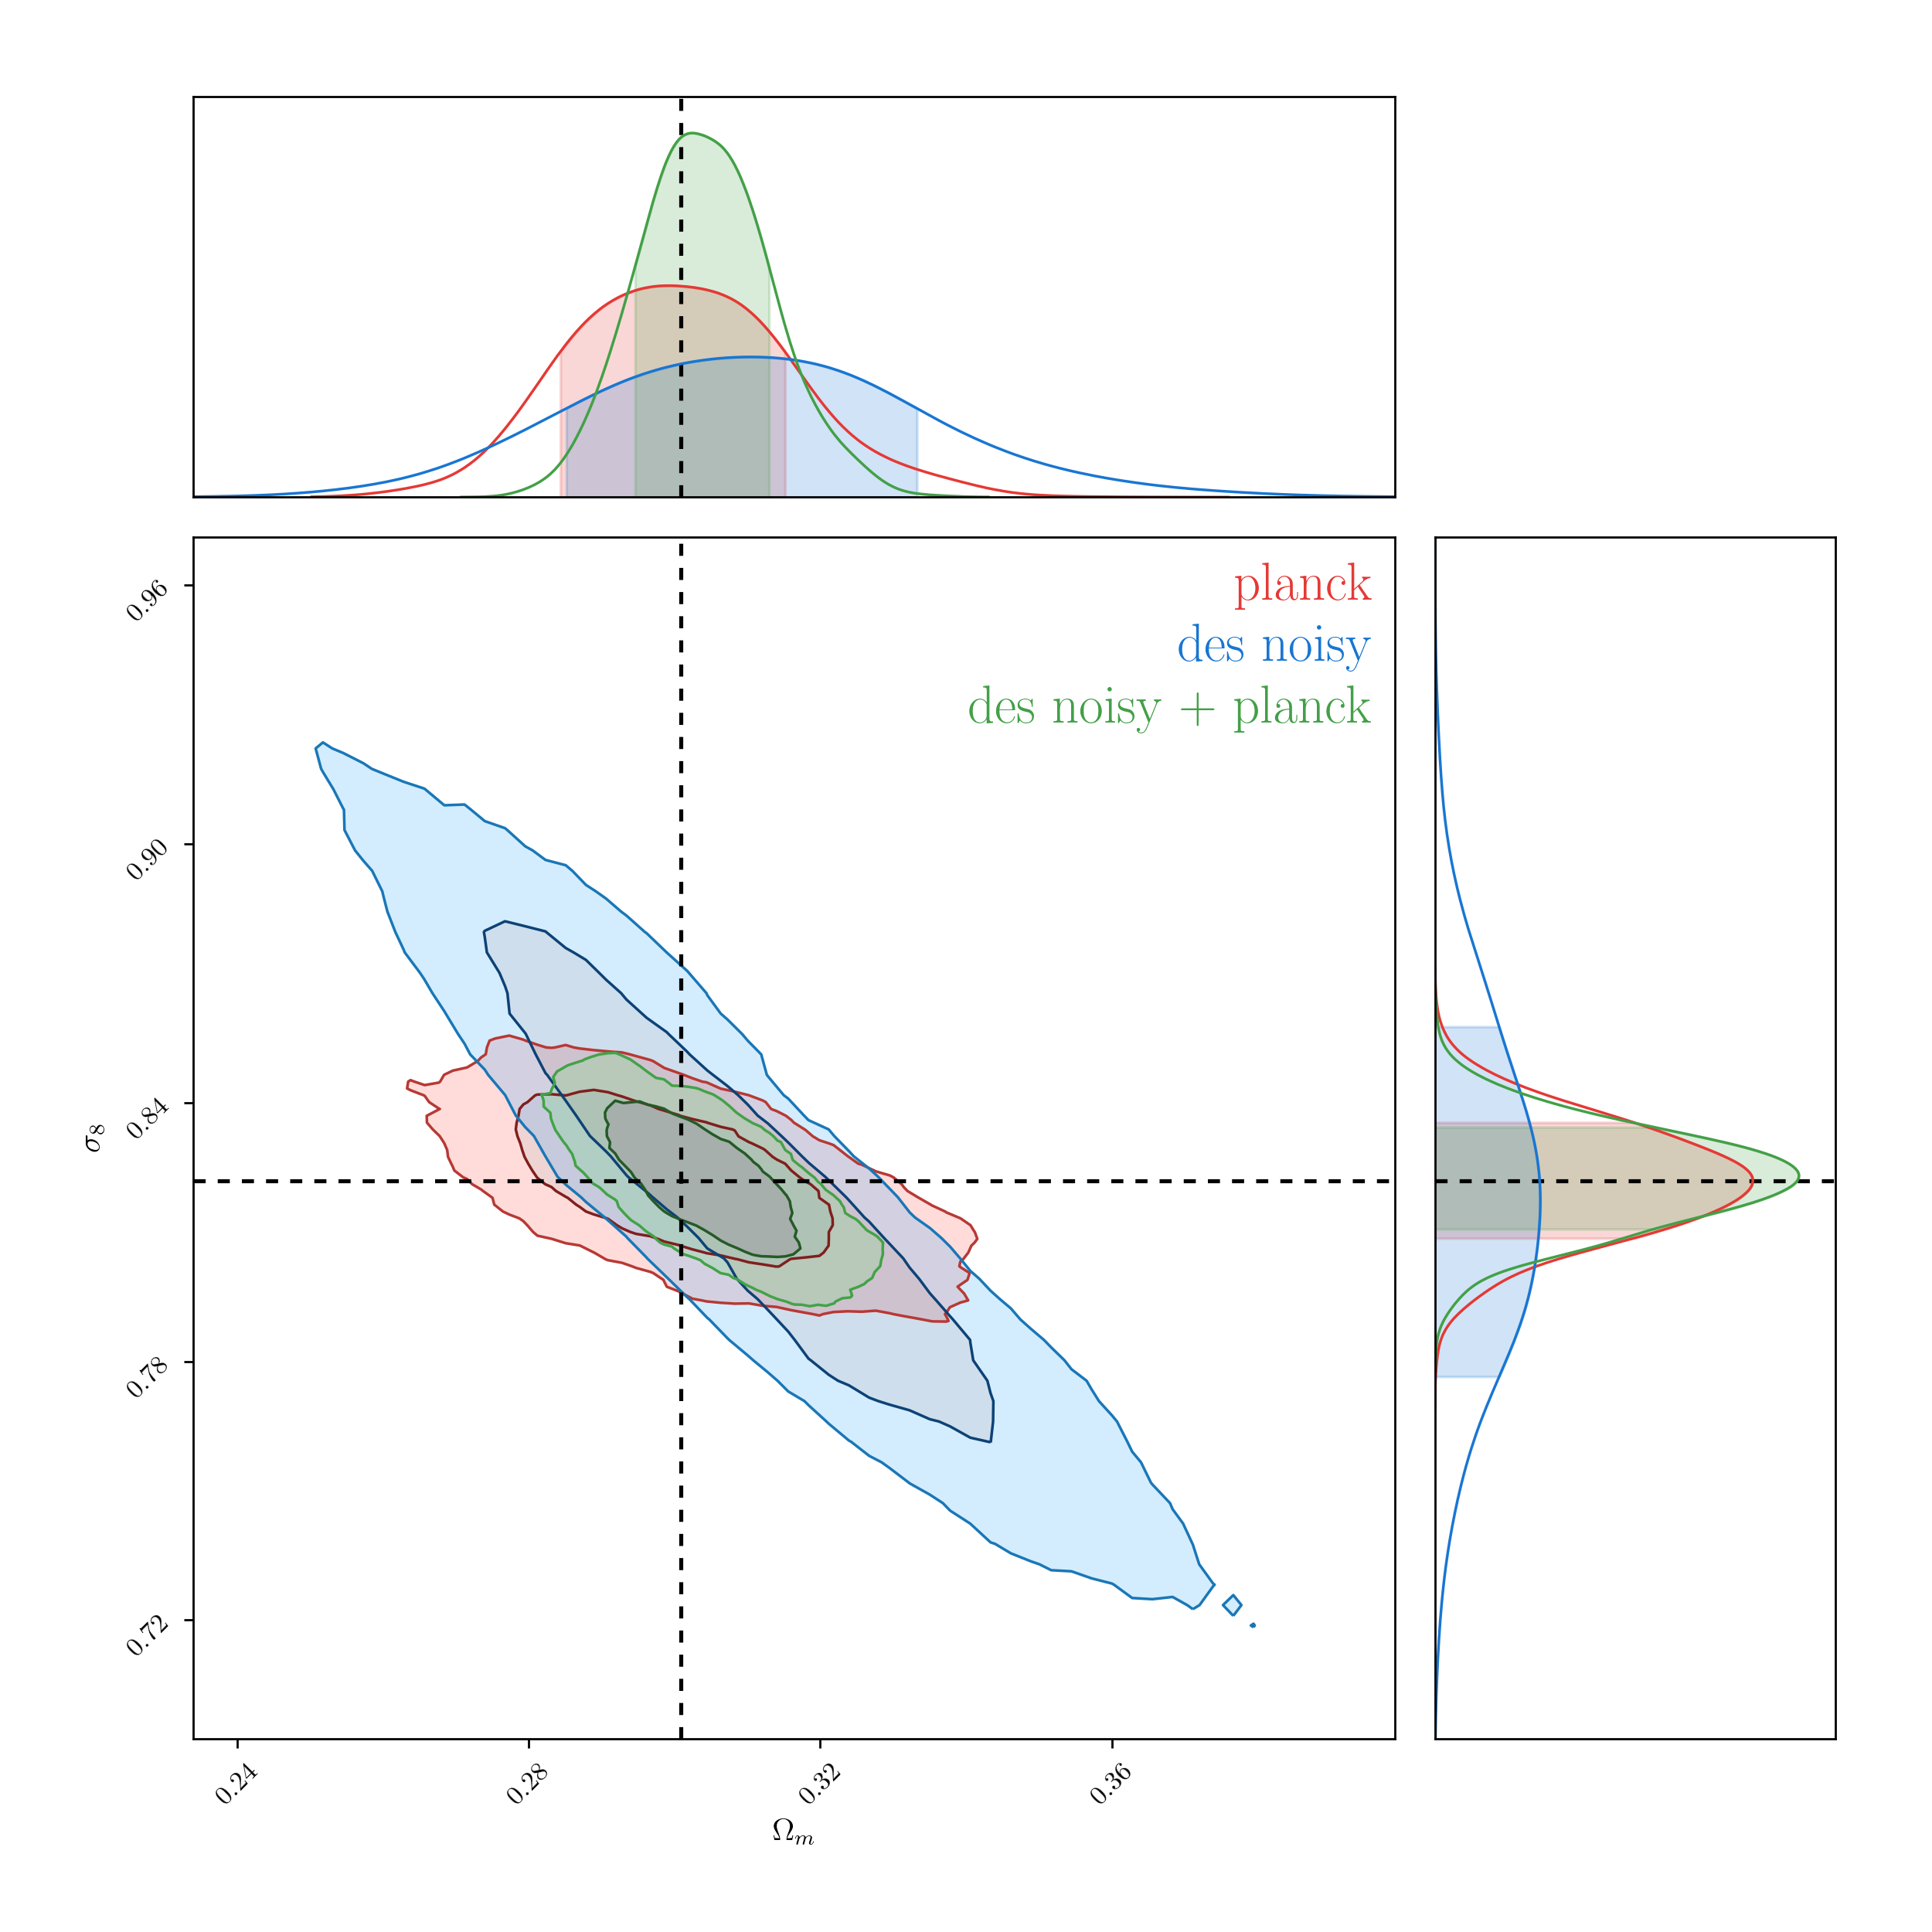
\includegraphics[height=12cm]{des+planck_poly2D.png}
\end{center}
 \caption{Posterior of Planck likelihood, red, DES 3x2pt simulated data, blue, and the combination of Planck and DES, green.}
\label{figure1}
\end{figure}

We are on the stage in which these simulated data-vectors then need to be run through the DES 3x2pt pipeline and through the combined DES+Planck pipeline to obtain the posterior and estimate the evidence in each case. 

\subsection{Anisotropic Clustering on Simulations}
I will basically download and read N-Body simulation data from \url{https://www.cosmosim.org}; precisely, we will need to use positions of approximately $1/100$ particles from HugeMDPL simulation at a snapshot of redshift $z=0$, which is a N-Body simulation with Planck cosmology, box size $4000 \, \rm  Mpc/h$ and $4096^3$ particles in total. Since the overall dataset is too large and we only need to use a fraction of it, my main goal is to download part of the data we need from this website and save to our own text format. We will simply use readgadget function from python package and select certain columns of data (position data) we need every 100 rows and save to three text files restoring x, y and z position respectively. Once we have these three files, we can do the rest computation on our own laptop.\\
The overall data of snapshot $z=0$ has a size of $1.7$ Tb. The Leibniz-Institute for Astrophysics Potsdam in collaboration with the MultiDark consortium created the MultiDark Database including HugeMDPL. Format of the files is gadget binary file. \\
We will use $wget$ to download these files. I am a registered user of \url{https://www.cosmosim.org} so I have the permission to download these data, and if we can form a paper out of these data, we will cite Klypin A., Yepes G., Gottl{\"o}ber S., Prada F., He{\ss} S., 2016, MNRAS, 457, 4340 and give credits to this database.


\section{Proposed Analyses and Justification of Requested Resources}

\section{Computational Resources}

\section{Research Plan}

\section{Grant Support}

\section{Total Allocation Request}

Our total request is:

{\bf 1,000,000 SUs on Bridges}

{\bf 10 PetaBtyes of storage}

\end{small}

%\newpage

\bibliographystyle{plain}
\bibliography{refs}

\end{document}
